\usetikzlibrary{shapes.geometric}
\usetikzlibrary{positioning}

\newcommand{\apparatus}[4]{\node[square node] (#1) at (#2,#3){#4};
                           \node[port] (#1+) at (#2 + 0.375, #3 + 0.5){+};
                           \node[port] (#1-) at (#2 + 0.375, #3 - 0.5){-};}

\part{Stern-Gerlach Experiments}

\chapter{Postulates}

To discuss Stern-Gerlach experiments, we first consider the mathematical objects used to model physical systems and variables. By comparing the objects used in classical and quantum mechanics, we make sense of the first three postulates of quantum mechanics. Then, we compare standard and consistent descriptions of spin measurement, and their relation to the fourth and fifth postulates.

\section{State Spaces and Physical Variables}
Consider the spin (intrinsic angular momentum) of an electron. Our system is the electron, and the classical spin state is simply a vector $S = (S_x, S_y, S_z)$ in $\mathbb{R}^3$, where each component $S_w$ is a physical variable that represents the magnitude of spin in the $w$ direction. Consequently, the components of spin state are mutually independent, and they can take on any real value. In other words, the sample spaces for each component are compatible, continuous and infinitely large. Because of the compatibility of spin component sample spaces, succesive observations of $S_x$, $S_y$, and $S_z$ uniquely determine the spin state.

Our physical variable of interest is the magnitude of spin in the $z$ direction; clasically, this variable is modeled by a function of spin state: $S_z(S) = \braket{z|S}$. This function relies on the inner product of the state space $\mathbb{R}^3$ to determine the magnitude of the spin vector in the $z$ direction only. In general, measurement of spin in three orthogonal directions uniquely determines the spin component in any direction $w$.

Experimental evidence raises issues with this classical description of spin states and $S_z$. First, only two values have ever been recorded, named \textit{spin-up} and \textit{spin-down}. These values are of equal magnitude $\frac{\hbar}{2}$ with positive and negative orientations, respectively. Second, the results of succesive measurements of a spin system impliy that the spin state is determined by spin along one axis only. Consequently, spin along more than one axis cannot be simultaneously determined; this is discussed further in section \ref{Section:Measurement}. To resolve these issues, we must change the mathematical objects used to represent system states and physical variables. Specifically, the sample space must restrict observed $S_w$ values to spin up and spin down, and the inability of determining spin in more than one direction should be reflected through incompatible sample spaces.

The quantum mechanical system state is described by a normalized vector in a linear state space. In fact, this is the first postulate of quantum mechanics:
\begin{Thm:Postulate}{1}
    The state of a physical system is defined by specifying an abstract vector $\ket{\psi}$ in a Hilbert state space $\mathcal{H}$.
\end{Thm:Postulate}

For spin-$\frac{1}{2}$ systems, the state space consists of all linear combinations of spin-up and spin-down:
\begin{equation}
    \mathcal{H} = \{\alpha\ket{+} + \beta\ket{-}\}
\end{equation}
where $\alpha, \beta \in \mathbb{C}$

For ease of calculation, we only consider normalized states, as scalar multiples of any normalized state bear the same physical meaning. We require $\alpha^2 + \beta^2 = 1$.

Defining system states in this way has dramatic consequences. A state includes all information that can be known about a system. A classical spin state includes spin magnitude in $x$, $y$, and $z$. The quantum state is only capable of determining spin magintude in one general direction $w$; spin in other directions not parallel or antiparallel to $w$ is undefined.

The second posulate of quantum mechanics states that physical variables are described by linear operators:
\begin{Thm:Postulate}{2}
    Every physical variable $\mathcal{A}$ is described by an operator $A$ acting in $\mathcal{H}$.
\end{Thm:Postulate}

Justifying the second postulate is easiest when also considering the third postulate:
\begin{Thm:Postulate}{3}
    The only possible result of the measurement of a physical variable $\mathcal{A}$ is one of the eigenvalues of the corresponding operator $A$.
\end{Thm:Postulate}

The operator correlates elements of a finite sample space (eigenvalues) with particular system states (eigenstates). Consequently, a state can only be interpreted as having a definite variable value if it is an eigenstate of the variable's operator. To illustrate this, consider the operator representing $S_z$. Written in its own basis,
\begin{align*}
    S_z \doteq \frac{\hbar}{2}\begin{bmatrix} 1 & 0 \\ 0 & -1 \end{bmatrix}
\end{align*}
This operator correlates $z$ spin-up $\left(S_z = \frac{\hbar}{2}\right)$ with
\begin{align*}
    \ket{\psi} = \ket{+}_z \doteq \begin{bmatrix} 1 \\ 0 \end{bmatrix}
\end{align*}
and $z$ spin-down $\left(S_z = \frac{-\hbar}{2}\right)$ with
\begin{align*}
    \ket{\psi} = \ket{-}_z \doteq \begin{bmatrix} 0 \\ 1 \end{bmatrix}
\end{align*}
Similarly, the operator representing $S_y$ written in the $S_z$ basis is
\begin{align*}
        S_y \doteq \frac{\hbar}{2}\begin{bmatrix} 0 & -i \\ i & 0 \end{bmatrix}
\end{align*}
This operator correlates $y$ spin-up $\left(S_y = \frac{\hbar}{2}\right)$ with
\begin{align*}
    \ket{\psi} = \ket{+}_y \doteq \frac{1}{\sqrt{2}}\begin{bmatrix} 1 \\ i \end{bmatrix}
\end{align*}
and $y$ spin-down $\left(S_y = \frac{-\hbar}{2}\right)$ with
\begin{align*}
    \ket{\psi} = \ket{-}_y \doteq \frac{1}{\sqrt{2}}\begin{bmatrix} 1 \\ -i \end{bmatrix}
\end{align*}

Operators for $S_z$ and $S_y$ share no common eigenstates, so no state can posses definite values for both variables. In general, operators for any spin component $S_j$, where $j$ is some direction not parallel or antiparallel with $z$, share no common eigenstates with $S_z$; in other words, $S_z$ and $S_j$ have incompatible sample spaces. By representing physical variables with an operator rather than a function, sample spaces become quantized and can be incompatible with each other. These features are necessary for predicting experimental results.

The first three postulates designate the mathematical objects used to model physical system states and variables. Consistent quantum theory does not modify these postulates; we will see that all of the strange features unique to quantum systems are a consequence of these postulates.

\section{Measurement}
\label{Section:Measurement}

In standard quantum mechanics, the fifth postualte (known as the projection postulate) describes how a system changes upon measurement. Defined as ``an interaction with a classical apparatus'', measurement instantaneously changes the measured state to the eigenstate corresponding to the measruement result.

\begin{Thm:Postulate}{5}
    If the measurement of the physical variable $\mathcal{A}$ on the system in the state $\ket{\psi}$ gives the result $a_n$, the state of the system immediately after the measurement is the normalized projection
    \begin{align*}
        \ket{\psi}^\prime = \frac{P_n\ket{\psi}}{\sqrt{\bra{\psi}P_n\ket{\psi}
        }}
    \end{align*}
    onto the subspace associated with $a_n$.
\end{Thm:Postulate}

Consider a measurement result for the $z$ component of spin, $S_z$. We represent the result with $n_z$, which could be either spin-up or spin-down. ${P^n}_z = \ket{n}_z\tensor[_z]{\bra{n}}{}$ is the projection operator for the state $\ket{n}_z$ corresponding to $n_z$. The new state is the projection of $\ket{\psi}$ onto $\ket{n}_z$, divided by the magnitude of that projection. The end result is that $\ket{\psi}$ becomes the normalized state $\ket{n}_z$. This process is known as \textit{state collapse} or \textit{wavefunction collapse}.

\begin{figure}
\centering\CaptionFontSize
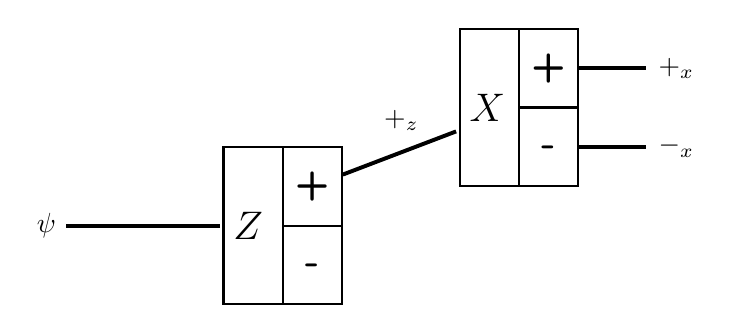
\begin{tikzpicture}[shorten >=1pt,auto, thick,
     square node/.style={rectangle, minimum height=2cm, minimum width=1.50cm, text width = 1.25cm, draw, font=\sffamily\Large\bfseries},
     port/.style={rectangle, draw,  minimum height=1cm, minimum width=0.75cm, font=\sffamily\Large\bfseries},
     wf/.style={rectangle, minimum height=1cm}]
    \apparatus{1}{3}{0}{$Z$};
    \apparatus{2}{6}{1.5}{$X$};

    \node[wf] (w0) at (0,0) {$\ket{\psi}$};
    \node[wf] (w1) at (8, 2.0) {$\ket{+}_x$};
    \node[wf] (w2) at (8, 1.0) {$\ket{-}_x$};

    \draw[line width=0.5mm] (w0) -- (1);

    \draw[line width=0.5mm] (1+) -- (2) node [near end] {$\ket{+}_z$};

    \draw[line width=0.5mm] (2+) -- (w1);
    \draw[line width=0.5mm] (2-) -- (w2);
\end{tikzpicture}
\caption[Insert an abbreviated caption here to show in the List of Figures]
{Demonstrating renormalizing upon measurment in standard quantum mechanics}
\label{Figure:Measurement:Renormalizing}
\end{figure}

As an example, consider the system shown in \fref{Figure:Measurement:Renormalizing}. The first apparatus serves as a state preparation device, since we are only interested in particles exiting the spin-up output. Using the projection postulate, the state after the first measurement is
\begin{align*}
    \ket{\psi_{top}} &= \frac{{P^z}_+\ket{\psi}}{\sqrt{\bra{\psi}{P^z}_+\ket{\psi}}} = \ket{+}_z
\end{align*}
Similarly, the possible output states from the second apparatus are
\begin{align*}
    \ket{\psi_{top}} &= \frac{{P^x}_+\ket{+}_z}{\sqrt{\bra{+}{P^x}_+\ket{+}_z}} = \ket{+}_x \\ \\
    \ket{\psi_{bottom}} &= \frac{{P^x}_-\ket{+}_z}{\sqrt{\bra{+}{P^x}_-\ket{+}_z}} = \ket{-}_x
\end{align*}

In consistent quantum theory, what is meant by ``measurement'' in the projection postulate is itself modeled as a physical process. Therefore, no notion of ``interaction with a classical apparatus'' is required to describe how states evolve when their classical properties are recorded. To describe measurement, each Stern-Gerlach apparatus has its own detector state space, containing orthonormal states representing each measurement result. For a Stern-Gerlach apparatus, a detection state is defined by a particle being located at some spatially separated output. In general, a detection state is some classical indicator; examples include an apparatus needle pointing up, or a particle colliding with a screen in a distinguishable region.

Let the state space of the $z$ apparatus be represented by
\begin{align*}
    {\mathcal{H}_D}_z =  \{\ket{D_+}_z, \ket{D_-}_z\}
\end{align*}
where
\begin{align*}
    _z\braket{D_+|D_+}_z&=1 \\
    _z\braket{D_+|D_-}_z&=0
\end{align*}
${\mathcal{H}_D}_x$ is similarly defined. Each detector state space is a subset of a global detector state space $\mathcal{H}_D$, so that we can require orthogonality of states in seperate dector spaces:
\begin{align*}
    _z\braket{D_n|D_m}_x=0 \\
    & \forall \ket{D_n}_z \in {\mathcal{H}_D}_z \\
    & \forall \ket{D_m}_x \in {\mathcal{H}_D}_x
\end{align*}

The act of measurement is described by correlating detector states with quantum states. The system then evolves by
\begin{align}
    \nonumber V: \\
    & \ket{\psi} = \left(\sum_{n} {P^z}_n\ket{\psi}\right) \otimes \left(\sum_{m} P_m\ket{D}\right) \mapsto \sum_{n} {P^z}_n\ket{\psi} \otimes \ket{D_n}
\end{align}
where ${P^z}_n$ is the projection operator for the $n^{th} z$ spin eigenstate and $P_m$ is the projection operator for the $m^{th}$ detector state.

This evolution describes a change in the eigenstates of the system. Before, $\ket{\psi}$ was a superposition of the tensor products of any spin eigenstate and any detector state. Any detector state could be realized with any quantum state. Afterwards, $\ket{\psi}$ is a superposition of the tensor products of a spin eigenstate and one specific detector state; a detector state can be realized with one specific quantum state only.

\fref{Figure:Measurement:DetectorStates} illustrates this description of measurement. The state of a particle leaving each output is the tensor product of a spin eigenstate and a detection state. As the quantum state is realized in incompatible sample spaces ($S_z$ and $S_x$), it loses information about its history; by posessing a definite $S_x$ value, information about $S_z$ is lost. However, the detector states are not impacted by these measurements, and the \textit{event history} of the state is preserved.

\begin{figure}
\centering\CaptionFontSize
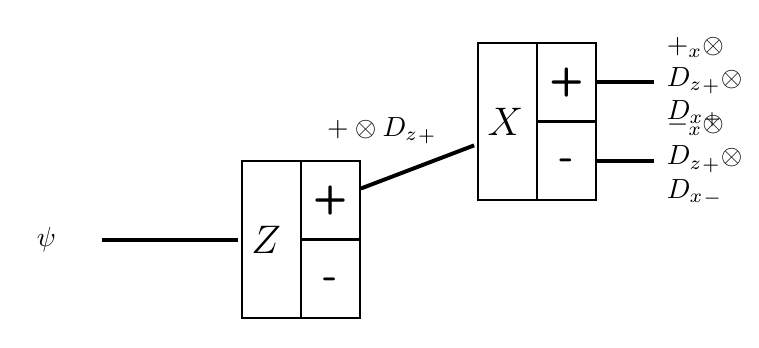
\begin{tikzpicture}[shorten >=1pt,auto, thick,
     square node/.style={rectangle, minimum height=2cm, minimum width=1.50cm, text width = 1.25cm, draw, font=\sffamily\Large\bfseries},
     port/.style={rectangle, draw,  minimum height=1cm, minimum width=0.75cm, font=\sffamily\Large\bfseries},
     wf/.style={rectangle, minimum height=1cm, text width = 0.7cm}]
    \apparatus{1}{3}{0}{$Z$};
    \apparatus{2}{6}{1.5}{$X$};

    \node[wf] (w0) at (0,0) {$\ket{\psi}$};
    \node[wf] (w1) at (8, 2.0) {$\ket{+}_x \otimes \ket{D_z}_+  \otimes \ket{D_x}_+$};
    \node[wf] (w2) at (8, 1.0) {$\ket{-}_x \otimes \ket{D_z}_+ \otimes \ket{D_x}_-$};

    \draw[line width=0.5mm] (w0) -- (1);

    \draw[line width=0.5mm] (1+) -- (2) node [near end] {$\ket{+} \otimes \ket{D_z}_+$};

    \draw[line width=0.5mm] (2+) -- (w1);
    \draw[line width=0.5mm] (2-) -- (w2);
\end{tikzpicture}
\caption[Insert an abbreviated caption here to show in the List of Figures]
{Demonstrating description of measurment as an abstract physical process in consistent quantum mechanics}
\label{Figure:Measurement:DetectorStates}
\end{figure}

% Measurment is now described by an abstract physical process. In this model, it is now feasible for state collapse to occur independent of physicists conducting clever experiments. For this sytem, we defined a detector state as a Stern Gerlach apparatus recording spin up or spin down. However, one could define detector states as any record of quantum systems possesing physical properties that interact with the classical world accordingly. Detector states describe a system's behavior classically without necessarily including any classical measurement apparatus.

\section{The Born Rule}

% Both probability and projection postulates relied on the term "measurement" in their definitions.  Using the probability postulate, the probabilities of each state leaving the Stern-Gerlach device oriented along the x-axis are
% \begin{align*}
%     \mathcal{P}_{+_x} &= |_x\braket{+|+}|^2 = \frac{1}{2} \\
%     \mathcal{P}_{-_x} &= |_x\braket{-|+}|^2 = \frac{1}{2}
% \end{align*} \\ TODO: introduce measurement problem.

We begin by comparing standard and consistent descriptions of measuring a quantum states' spin along one axis using a Stern-Gerlach apparatus.

We accept the first three postulates of quantum mechanics.

\begin{enumerate}
    \item All information known about a quantum mechanical system is represented by an abstract vector $\ket{\psi}$. This vector lives in a linear state space $\mathcal{H}$, which is the set of all possible states of the quantum system.
    \item A physical observable of the system is represented by a linear operator $A$ that acts on vectors in $\mathcal{H}$.
    \item The only possible measurement results of a physical observable are the eigenvalues $a_n$ of the corresponding observable $A$.
\end{enumerate}

We accept the second and thirst postulates because they do not describe the operator's relationship to the measurement process. The second correlates a measurable quantity of the system to an operator, while the third describes the possible results. However, care must be taken when interpreting a "measurement result of $a_n$". We take this to mean that some record exists of the system behaving classically such that $A$ must have been $a_n$.

The fourth and fifth postulates require more scrutiny. In standard quantum mechanics, the act of measurement plays a special role in assigning probabilities to measurement outcomes through the probability postulate, and in determmining the evolution of the state through the projection postulate.

The probability postulate assigns probabilities to each measurement result by taking the inner product of $\ket{\psi}$ and the eigenstate $\ket{n}$ corresponding to measurement result $n$:
\begin{align}
    \mathcal{P}_n = |\braket{n|\psi}|^2
\end{align}

This postulate is also known as the \textit{Born Rule}, which is usually presented in the language of wavefunctions. The probability that a system is found at position $x$ is
\begin{align}
    \mathcal{P}_x = |\psi(x)|^2
\end{align}
which follows from the wavefunction's definition as the inner product of the $\ket{x}$ eigenstate and $\psi$.



To compute probabilities of each outcome, we introduce an analog of the Born Rule: sum the magnitudes of each branch wavefunction that includes the corresponding detector state. This is accomplished by finding the trace of the projection operator of that detector state acting on the projection operator or the overall evolved state.
\begin{align}
    \mathcal{P}_n = Tr(P^D_n \cdot V\ket{\psi}\bra{\psi}V^\dagger)
\end{align}

TODO: explain trace

In this simple Stern-Gerlach example, there is only one branch wavefunction correlated with each detector state. So, computing probabilities is done by finding the magnitude of each branch wavefunction.

TODO: compute probabilities, show it is equal to std QM

\Chapter{Complementarity}

We now compare standard and consistent quantum mechanics' treatment of the principle of complementarity. Arguably the most fundamental feature of quantum mechanics, the principle of complementarity states that a quantum system has pairs of physical observables which cannot be measured simultaneously. Components of spin on orthogonal axes are complementary properties, so we examine measurements of succesive Stern-Gerlach experiments. We will see how complementarity is a strange consequence of the standard postulates of quantum mechanics, while in consistent formulations, complementarity is itself a postulate from which strange consequences arise.

First, we compute the probabilities of each outcome using standard quantum mechanics. The first apparatus serves as a state preparation device with output $\ket{+}$. By the direction of the projection postulate, the state is renormalized upon each measurement. After measuring a property complementary to what is known (such as spin along $x$, knowing spin along $z$), any information known about the input state is lost; the input state instantaneously changes to the state corresponding to the observed quantity. Consequently, there is an equal probability of observing the final state as $\ket{+}$ or $\ket{-}$ at either final apparatus, even though the state was initially prepared as $\ket{+}$, since
\begin{align*}
    \mathcal{P}_n &= |\braket{+|+}_x|^2 \\
                  &= |\braket{-|+}_x|^2 \\
                  &= |\braket{+|-}_x|^2 \\
                  &= |\braket{-|-}_x|^2 \\
                  &= \frac{1}{4}
\end{align*}
This contradiction with classical intuition is a direct result of the projection postulate. The act of measurement causes the system to shed properties previously recorded. TODO: describe measurement problem.

TODO: Demonstrate complementarity and single framework rule

\begin{figure}
\centering\CaptionFontSize
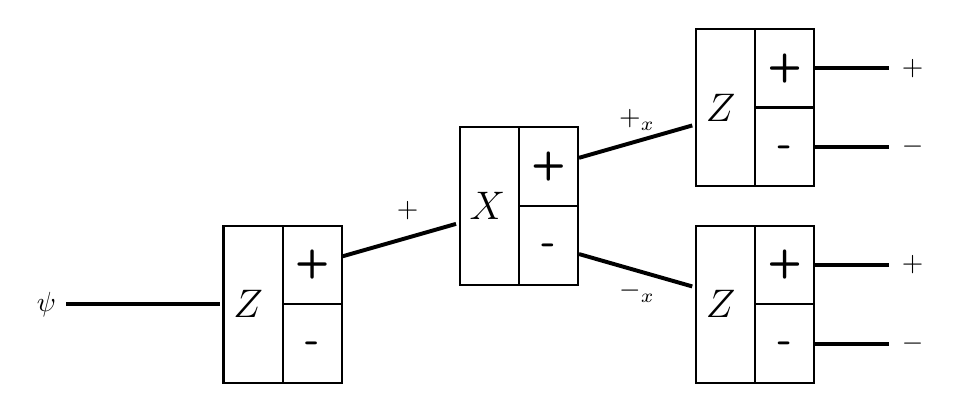
\begin{tikzpicture}[shorten >=1pt,auto, thick,
     square node/.style={rectangle, minimum height=2cm, minimum width=1.50cm, text width = 1.25cm, draw, font=\sffamily\Large\bfseries},
     port/.style={rectangle, draw,  minimum height=1cm, minimum width=0.75cm, font=\sffamily\Large\bfseries},
     wf/.style={rectangle, minimum height=1cm}]
    \apparatus{1}{3}{0}{$Z$};
    \apparatus{2}{6}{1.25}{$X$};
    \apparatus{3}{9}{2.50}{$Z$};
    \apparatus{4}{9}{0}{$Z$};

    \node[wf] (w0) at (0,0) {$\ket{\psi}$};
    \node[wf] (w1) at (11, 3.0) {$\ket{+}$};
    \node[wf] (w2) at (11, 2.0) {$\ket{-}$};
    \node[wf] (w3) at (11, 0.5) {$\ket{+}$};
    \node[wf] (w4) at (11, -0.5) {$\ket{-}$};

    \draw[line width=0.5mm] (w0) -- (1);

    \draw[line width=0.5mm] (1+) -- (2) node [near end] {$\ket{+}$};

    \draw[line width=0.5mm] (2-) -- (4) node [midway, below] {$\ket{-}_x$};
    \draw[line width=0.5mm] (2+) -- (3) node [midway, above] {$\ket{+}_x$};

    \draw[line width=0.5mm] (3-) -- (w2);
    \draw[line width=0.5mm] (3+) -- (w1);
    \draw[line width=0.5mm] (4-) -- (w4);
    \draw[line width=0.5mm] (4+) -- (w3);
\end{tikzpicture}
\caption[Insert an abbreviated caption here to show in the List of Figures]
{Demonstrating complementary measurments in standard quantum mechanics}
\label{Figure:Intro:FigureExampleC}
\end{figure}

\begin{figure}
\centering\CaptionFontSize
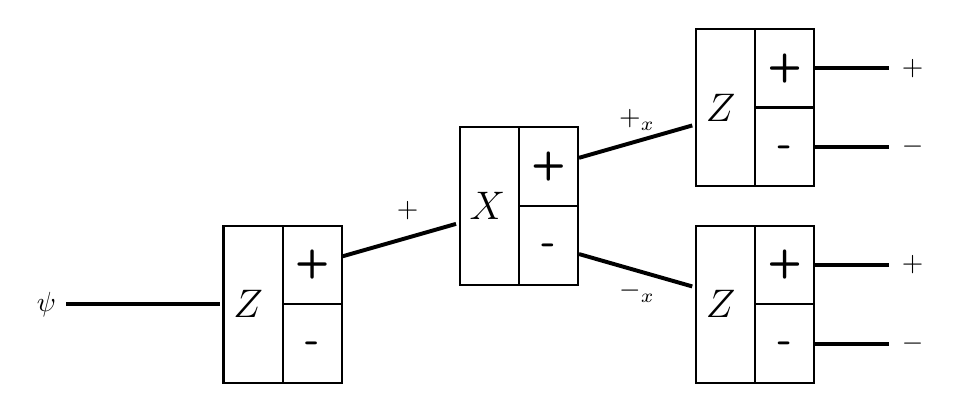
\begin{tikzpicture}[shorten >=1pt,auto, thick,
     square node/.style={rectangle, minimum height=2cm, minimum width=1.50cm, text width = 1.25cm, draw, font=\sffamily\Large\bfseries},
     port/.style={rectangle, draw,  minimum height=1cm, minimum width=0.75cm, font=\sffamily\Large\bfseries},
     wf/.style={rectangle, minimum height=1cm}]
    \apparatus{1}{3}{0}{$Z$};
    \apparatus{2}{6}{1.25}{$X$};
    \apparatus{3}{9}{2.50}{$Z$};
    \apparatus{4}{9}{0}{$Z$};

    \node[wf] (w0) at (0,0) {$\ket{\psi}$};
    \node[wf] (w1) at (11, 3.0) {$\ket{+}$};
    \node[wf] (w2) at (11, 2.0) {$\ket{-}$};
    \node[wf] (w3) at (11, 0.5) {$\ket{+}$};
    \node[wf] (w4) at (11, -0.5) {$\ket{-}$};

    \draw[line width=0.5mm] (w0) -- (1);

    \draw[line width=0.5mm] (1+) -- (2) node [near end] {$\ket{+}$};

    \draw[line width=0.5mm] (2-) -- (4) node [midway, below] {$\ket{-}_x$};
    \draw[line width=0.5mm] (2+) -- (3) node [midway, above] {$\ket{+}_x$};

    \draw[line width=0.5mm] (3-) -- (w2);
    \draw[line width=0.5mm] (3+) -- (w1);
    \draw[line width=0.5mm] (4-) -- (w4);
    \draw[line width=0.5mm] (4+) -- (w3);
\end{tikzpicture}
\caption[Insert an abbreviated caption here to show in the List of Figures]
{Demonstrating complementary measurments in consistent quantum mechanics}
\label{Figure:Intro:FigureExampleD}
\end{figure}

\begin{figure}
\centering\CaptionFontSize
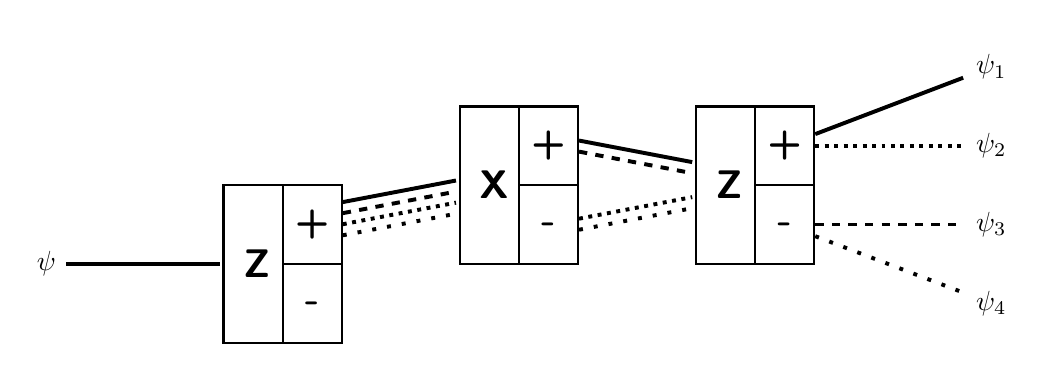
\begin{tikzpicture}[shorten >=1pt,auto, thick,
     square node/.style={rectangle, minimum height=2cm, minimum width=1.50cm, text width = 1cm, draw, font=\sffamily\Large\bfseries},
     port/.style={rectangle, draw,  minimum height=1cm, minimum width=0.75cm, font=\sffamily\Large\bfseries},
     wf/.style={rectangle, minimum height=1cm}]
    \apparatus{1}{3}{0}{Z};
    \apparatus{2}{6}{1}{X};
    \apparatus{3}{9}{1}{Z};

    \node[wf] (w0) at (0,0) {$\ket{\psi}$};
    \node[wf] (w1) at (12,2.5) {$\ket{\psi_1}$};
    \node[wf] (w2) at (12,1.5) {$\ket{\psi_2}$};
    \node[wf] (w3) at (12,0.5) {$\ket{\psi_3}$};
    \node[wf] (w4) at (12,-0.5) {$\ket{\psi_4}$};

    \draw[line width=0.5mm] (w0) -- (1);

    \draw[transform canvas={yshift=-0.6em}, line width=0.5mm, loosely dotted] (1+) -- (2);
    \draw[transform canvas={yshift=-0.2em}, line width=0.5mm, dotted] (1+) -- (2);
    \draw[transform canvas={yshift=0.2em}, line width=0.5mm, dashed] (1+) -- (2);
    \draw[transform canvas={yshift=0.6em}, line width=0.5mm] (1+) -- (2);

    \draw[transform canvas={yshift=-0.4em}, line width=0.5mm, loosely dotted] (2-) -- (3);
    \draw[transform canvas={yshift=0em}, line width=0.5mm, dotted] (2-) -- (3);
    \draw[transform canvas={yshift=0em}, line width=0.5mm, dashed] (2+) -- (3);
    \draw[transform canvas={yshift=0.4em}, line width=0.5mm] (2+) -- (3);

    \draw[line width=0.5mm, loosely dotted] (3-) -- (w4);
    \draw[line width=0.5mm, dashed] (3-) -- (w3);
    \draw[line width=0.5mm, dotted] (3+) -- (w2);
    \draw[line width=0.5mm] (3+) -- (w1);
\end{tikzpicture}
\caption[Insert an abbreviated caption here to show in the List of Figures]
{TODO: create section to discuss this example, and how it creates an inconsistent set of histories. Describe how the set can be made to be consistent}
\label{Figure:Intro:FigureExampleE}
\end{figure}
